\ifdefined\standalone 
\documentclass[12pt]{article}
\usepackage{graphicx}
\usepackage{float}
\usepackage[a4paper, margin=1in]{geometry}
\usepackage[utf8]{inputenc}
\usepackage{textcomp}
\usepackage{amsmath}
\usepackage{booktabs}
\usepackage{tikz}
\usepackage{enumitem}
\usetikzlibrary{decorations.pathmorphing}
\usepackage[hidelinks]{hyperref} % <- hypertext

\begin{document}
\fi

\section{Reference Cone Calorimeter Configuration}

This validation case aims to assess the ability of Gpyro to reproduce a standard one-dimensional pyrolysis scenario representative of cone calorimeter tests, and to compare the results with those from the reference codes Thermakin and FDS, as detailed in the study~\cite{abdelhafiz2025}.

A fictitious but physically coherent material, referred to as \textbf{Material A}, is used. Two independent first-order chemical reactions are modeled using the kinetic parameters detailed in Table~\ref{tab:chem_props}, and the thermophysical properties of all solid species are provided in Table~\ref{tab:phys_props}.

The physical configuration consists of a 6~mm thick layer of Material A placed atop a 12~mm Kaowool insulation layer. A constant external heat flux of $50~\mathrm{kW/m^2}$ is applied to the top surface. Convective heat transfer is imposed with a heat transfer coefficient of $h_c = 8.2~\mathrm{W/m^2{\cdot}K}$ and an ambient temperature of $25~^\circ\mathrm{C}$. The bottom surface exchanges heat with the environment solely via thermal radiation. Figure~\ref{fig:ref_configuration} illustrates the configuration.

To ensure equivalence with the reference codes, the following modeling assumptions are adopted:

\begin{itemize}[noitemsep, topsep=0pt]
\item Gas-phase contributions to energy conservation are neglected.
\item Gas release is assumed to be instantaneous (no gas transport).
\item Reaction enthalpies are treated as constant.
\item No material deformation is modeled (densities chosen to preserve volume).
\end{itemize}

\vspace{1em} 

A uniform spatial discretization of 0.02~mm and a time step of 0.05~s are used. Numerical convergence is verified under these settings.

\begin{table}[H]
\centering
\caption{Chemical kinetics parameters}
\label{tab:chem_props}
\begin{tabular}{@{}llllll@{}}
\toprule
Reaction & $A_k$ ($\mathrm{s^{-1}}$) & $E_k$ ($\mathrm{kJ/mol}$) & $n_k$ (-) & $\Delta H_k$ ($\mathrm{J/kg}$) & $\theta_k$ ($\mathrm{kg/kg}$) \\
\midrule
A $\rightarrow$ $\theta_1$ B + (1$-\theta_1$) Gas$_1$ & $9.5 \times 10^{20}$ & 249 & 1 & $1.7 \times 10^5$ & 0.44 \\
B $\rightarrow$ $\theta_2$ C + (1$-\theta_2$) Gas$_2$ & $5.5 \times 10^{11}$ & 192 & 1 & $1.2 \times 10^6$ & 0.47 \\
\bottomrule
\end{tabular}
\end{table}

\begin{table}[H]
\centering
\caption{Thermophysical properties of solid species}
\label{tab:phys_props}
\begin{tabular}{@{}llllll@{}}
\toprule
Material & $k$ ($\mathrm{W/m{\cdot}K}$) & $c_p$ ($\mathrm{J/kg{\cdot}K}$) & $\rho$ ($\mathrm{kg/m^3}$) & $\alpha$ ($\mathrm{m^{-1}}$) & $\varepsilon$ (-) \\
\midrule
Material A & $0.17 + 3.10^{-4}T$ & 1550 & 1430 & $\infty$ & 1.0 \\
Material B & $0.24 + 8.10^{-4}T$ & 1720 & 629.2 & $\infty$ & 1.0 \\
Material C & $0.36 + 18.10^{-4}T$ & 780  & 265.7 & $\infty$ & 1.0 \\
Kaowool    & 0.058               & 1070  & 256   & $\infty$ & 0.95 \\
\bottomrule
\end{tabular}
\end{table}

The results obtained using Gpyro are compared to those from Thermakin and FDS. Figure~\ref{fig:ref_MLR} presents the comparison of the Mass Loss Rate (MLR) profiles. Figure~\ref{fig:reference_cc_T} illustrates the evolution of temperature at various depths, while Figure~\ref{fig:reference_cc_concentration} shows the time-dependent evolution of species concentrations at a depth of 3~mm.
\begin{figure}[H]
\centering

\begin{minipage}[t]{0.45\textwidth}
\centering
\begin{tikzpicture}[scale=1.0]
\draw[fill=orange!20] (0,0) rectangle (6,0.6); % Material A
\draw[fill=gray!30] (0,-1.2) rectangle (6,0); % Kaowool

\node at (3,0.3) {Material A};
\node at (3,-0.6) {Kaowool};

\draw[<->] (-0.5,0) -- (-0.5,0.6);
\node[left] at (-0.5,0.3) {6~mm};

\draw[<->] (-0.5,-1.2) -- (-0.5,0);
\node[left] at (-0.5,-0.6) {12~mm};

\foreach \x in {1.8,2.8,3.8}
    \draw[->,thick,red] (\x+0.2,1.6) -- (\x+0.2,0.6);

\node[above,red] at (3,1.7) {$\dot{q}'' = 50~\mathrm{kW/m^2}$};

\draw[->,thick, blue] (6,0.8) -- (5,0.8) arc[start angle=90, end angle=360, radius=0.1cm]; 
\draw[->,thick, blue] (6,1) -- (5,1) arc[start angle=270, end angle=0, radius=0.1cm]; 

\node[blue] at (4.8,1.4) {\scriptsize $h_c = 8.2~\mathrm{W.m^{-2}{\cdot}K^{-1}$};
\node[blue] at (1,1) {\scriptsize $T_\infty = 25~^\circ\mathrm{C}$};

\foreach \x in {1.5,3,4.5}
    \draw[purple,thick,->,decorate,decoration={snake,amplitude=1mm,segment length=3mm}] (\x,-1.2) -- (\x,-1.8);

\node[below,purple] at (3,-1.7) {\scriptsize Radiative loss};
\end{tikzpicture}
\caption{Configuration schematic}
\label{fig:ref_configuration}
\end{minipage}
\hfill
\begin{minipage}[t]{0.48\textwidth}
\centering
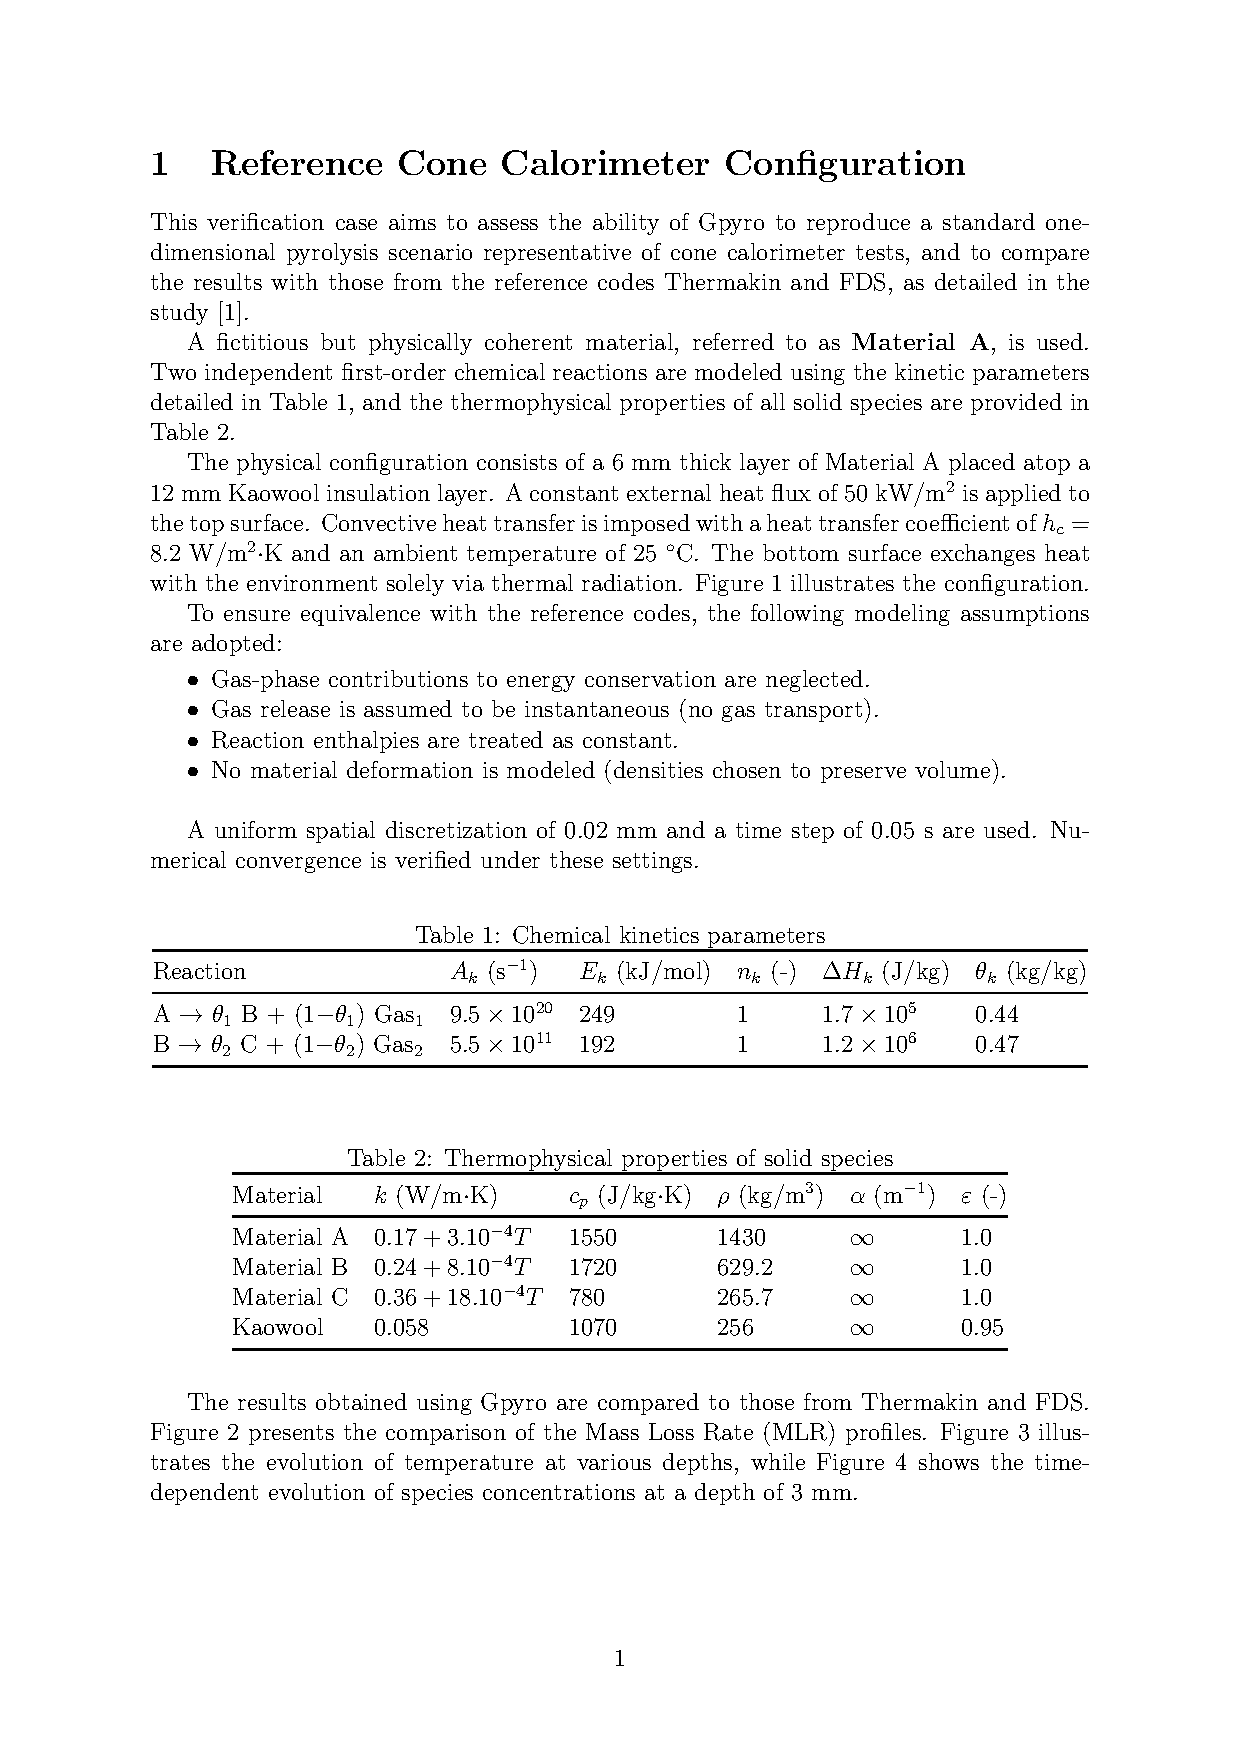
\includegraphics[width=\linewidth]{reference_cc.png}
\caption{Mass Loss Rate (MLR) comparison}
\label{fig:ref_MLR}
\end{minipage}

\end{figure}


\vspace{1em}

\begin{figure}[H]
\centering

\begin{minipage}[t]{0.48\textwidth}
\centering
\includegraphics[width=\linewidth]{reference_cc_T.png}
\caption{Temperature evolution at different depths}
\label{fig:reference_cc_T}
\end{minipage}
\hfill
\begin{minipage}[t]{0.48\textwidth}
\centering
\includegraphics[width=\linewidth]{reference_cc_Concentration.png}
\caption{Species concentration evolution at 3~mm depth}
\label{fig:reference_cc_concentration}
\end{minipage}

\end{figure}

\ifdefined\standalone
\bibliographystyle{unsrt}
\bibliography{reference_cc}
\end{document}
\fi






